 \chapter{Prehľad problematiky}\label{chap:issues_overview}

Prístup na určovanie pozície ruky môže byť rôzny v závislosti na vstupných dátach. Sú to obrázky buď z jednej kamery, RGB z viacerých zosynchronizovaných kamier alebo RGB-D. Keďže sa zaoberáme oblasťou interakcie robota s ľudským učiteľom, informácia v 3D priestore má prínos pre širšie vnímanie prostredia robotom. Táto informácia je poskytnutá iba pri RGB-D dátach a pri ostatných vstupoch je potrebné informáciu o hĺbke dopočítať. Týmto prístupom sa venovalo niekoľko prác, ktoré prichádzajú s riešeniami k problémom.

Táto časť obsahuje základné informácie, ktoré sú potrebné na pochopenie a prácu v danej problematike. Na úvod popíšeme základný princíp neurónových sietí, konvolučných sietí a ich niektorých vrstiev a popíšeme architektúru hourglass použitú v praktickej časti. Ďalej vysvetlíme 3 rôzne pohľady prístupov na riešenie našej problematiky. V závere tejto kapitoly uvedieme informácie o datasetoch a kamere použitej v praktickej časti.

\section{Neurónové siete}\label{chpt:neuralNetwork}
Myšlienka neurónových sietí vychádza z princípu výpočtov mozgu, ktorý funguje inak ako bežné počítače. Mozog je v podstate komplexný, nelineárne, paralelný počítač a má schopnosť udržať konzistentnú štruktúru neurónov. Dokáže vykonať isté výpočty mnohonásobne rýchlejšie ako najrýchlejší počítač.

Úlohou umelej neurónovej siete je modelovať riešenie problémov spôsobom podobným mozgu. Sieť je obvykle implementovaná elektronickými komponentami alebo je simulovaná softvérom. Je zložená z umelých neurónov a množstvom prepojení medzi nimi, často označovanými ako synaptické váhy. Druh sietí z ktorého vychádzajú aj konvolučné neurónové siete popísané v sekcii \ref{CNN} využíva proces učenia na to, aby boli ich výsledky použiteľné. Učenie je v tejto oblasti reprezentované funkciou, ktorá upravuje váhy siete tak, aby minimalizovala rozdiel medzi požadovaným výstupom a výstupom z neurónovej siete. Takáto sieť je ilustračne znázornená na obr. \ref{img:11NN}, kde sú čiernymi šípkami znázornené synaptické váhy.

\begin{figure}[H]
	\begin{center}
		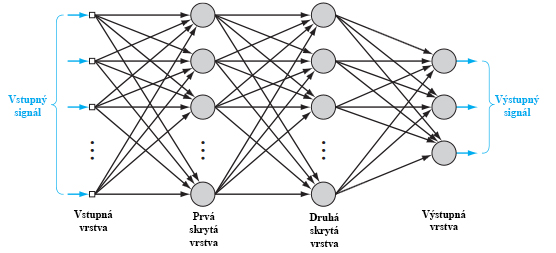
\includegraphics[width=\textwidth]{images/11NN.jpg}
		\caption{Graf siete s architektúrou zvanou viacvrstvový perceptrón \cite{haykin2009neural}. }
		\label{img:11NN}
	\end{center}
\end{figure}

% Definícia neurónovej siete ako adaptívny stroj podľa Haykin a kol. \cite{haykin2009neural}:
% \theoremstyle{definition}
% \newtheorem{definition}{Definícia}[section]
% \begin{definition}{Neurónová sieť}
%     \emph{ 
%     Neurónová sieť je paralelný distribuovaný procesor zložený z jednoduchých procesných jednotiek, ktoré prirodzene uchovávajú vedomosť so skúseností a sú schopné túto vedomosť použiť. Sú podobné mozgu v dvoch aspektoch:
%     \begin{enumerate}
%         \setlength\itemsep{0px}
%         \item Vedomosť je nadobudnutá v prostredí, kde nastáva učiaci proces.
%         \item Nadobudnutá vedomosť je uložená v spojeniach (synaptických váhach) medzi neurónmi.
%     \end{enumerate}
%     }
% \end{definition}
V tejto časti popíšeme jednoduchú sieť na klasifikáciu. Architektúra siete je ilustračne znázornená na obr. \ref{img:11NN}, kde vstupný signál je vektor príznakov, ktorý chceme klasifikovať. Výstupný signál predstavuje vektor ohodnotení, ktorý je vypočítaný zo vstupného signálu a aplikovaním dopredného výpočtu. Vektor ohodnotení vyjadruje určenie triedy, do ktorej patrí vstupný signál. Po určení triedy je vypočítaná chyba. Pri klasifikácii sa určí chyba podľa správnosti klasifikácie vstupného signálu ako počet správne klasifikovaných príkladov vydelený počtom všetkých príkladov. Výsledok vyjadruje chybu v percentách. Následne je aplikovaný proces učenia. Tento postup použitia sietí je nazývaný ako učenie s učiteľom \cite{haykin2009neural}.

\textbf{Dopredný výpočet} prebieha zo vstupného signálu cez všetky vrstvy a vypočíta výstupný signál. Smer výpočtu je znázornený čiernymi šípkami na obr. \ref{img:12backprop}. V tejto fáze sú váhy pevne dané a neupravujú sa. Vrstvy sú poprepájané tak, že výstup predchádzajúcej vrstvy je vstupom nasledujúcej vrstvy. Na každej vrstve prebieha nasledovný výpočet (\ref{feedforward}), kde $x_i$ je vstupom do vrstvy, $w_{ij}$ je váha medzi vstupom a neurónom, a $f$ je aktviačná funkcia ako napríklad $sigmoid, tanh, ReLU$.

\begin{equation}\label{feedforward}
    f\left( \sum{x_i \cdot w_{ij}} \right)
\end{equation}

\textbf{Proces učenia} využíva učiaci algoritmus, ktorý pracuje na princípe spätného šírenia chyby zvanom \textbf{back propagation} \cite{haykin2009neural}. Tento postup je smerovaný z výstupnej vrstvy, cez všetky skryté vrstvy až ku vstupnej. Smer je znázornený na obr. \ref{img:12backprop} modrými šípkami. Váhy sú upravené na každej vrstve podľa nasledovného výpočtu \cite{haykin2009neural}:

\begin{equation}\label{deltarule}
    w_{ji}(n) = w_{ji}(n)-\eta\frac{\partial{E(n)}}{\partial{w_{ji}(n)}}
\end{equation}

Kde $\eta$ je rýchlosť učenia, parciálna derivácia vyjadruje gradient a mínus preto, aby sme zmenšovali chybu, teda posunuli výsledok proti smeru gradientu. 
Chyba je vyjadrená priemerným rozdielom medzi očakávaným a predikovaným výstupom pre jednu dávku vstupných príkladov. Matematicky zapísané rovnicou:

\begin{equation}\label{eqn:SGDerror}
    {
        E(n) = \frac{1}{n}\sum_{i=1}^{n}{l(f(x) - y)}
    }
\end{equation}

Kde uvažujeme funkciu $f$, ktorá na základe váh vypočíta výstupnú hodnotu a funkciu $l$, ktorá definuje meranie vzdialenosti medzi očakávaným a predikovaným výstupom. Zvyčajne je počítaná ako euklidovská, prípadne tzv. Manhattanská vzdialenosť. Táto metóda sa nazýva \textbf{stochastic gradient descent} \cite{bottou-tricks-2012}.

\begin{figure}[H]
	\begin{center}
		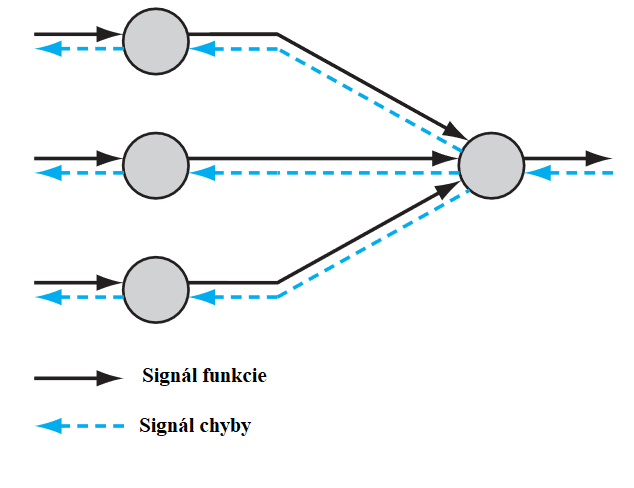
\includegraphics[height=180px]{images/12backprop.png}
		\caption{Ilustrácia dopredného (výpočet funkcie) a spätného (výpočet chyby) šírenia signálu \cite{haykin2009neural}. }
		\label{img:12backprop}
	\end{center}
\end{figure}

\section{Konvolučné siete} \label{CNN}
Konvolučné siete \cite{Goodfellow-et-al-2016} tiež nazývané  konvolučné neurónové siete alebo CNN sú špeciálnym typom neurónových sietí pre spracovanie dát, ktoré majú známu mriežkovú topológiu. Príkladom takýchto dát sú dáta v časovej sérii, ktoré sú reprezentované vo vektore s časovou informáciou. Ďalším príkladom sú obrázky reprezentované v matici (tenzore) pixelov. Názov naznačuje, že v takej sieti je použitá matematická operácia konvolúcia. Sú to teda neurónové siete, ktoré používajú konvolúciu pri všeobecnom maticovom násobení aspoň na jednej vrstve neurónovej siete. Konvolúcia je matematická operácia medzi dvoma funkciami s argumentami hodnôt na reálnych číslach. Môže byť definovaná \cite{Goodfellow-et-al-2016} spojitá (\ref{eqn:continuousConvolutionDefinition}) alebo diskrétna (\ref{eqn:discreteConvolutionDefinition}) konvolúcia, kde sú $x$ a $w$ funkciami a $a$, $t$ hodnotami reálnych čísel. Označuje sa hviezdičkou \ref{convolutionMarker}.
\begin{equation}\label{eqn:continuousConvolutionDefinition}
    {
        s(t) = \int{x(a)w(t-a)da}
    }
\end{equation}
\begin{equation}\label{eqn:discreteConvolutionDefinition}
    {
        s(t) = \sum_{a=-\inf}^{\inf}{x(a)w(t-a)}
    }
\end{equation}
\begin{equation}\label{convolutionMarker}
    {s(t) = (f*g)(t)}
\end{equation}
Kde $f$ a $g$ sú funkcie a $t$ je premenná na množine reálnych čísel. V terminológii konvolučných neurónových sietí je prvý argument (v tomto prípade $f$) konvolúcie označovaný ako vstup a druhý argument ($g$) ako {\bf jadro}. Výstup z konvolúcie je označením pre {\bf mapu príznakov}. Vstup je obvykle viacrozmerné pole dát a kernel viacrozmerné pole parametrov, ktorý sa upravuje počas učenia. Viacrozmerné polia nazývame tenzor.

  \subsection{Motivácia}
%Konvolúcia pokrýva tri dôležité oblasti, v ktorých je použitie konvolúcie značným prínosom.
Využtie operácie konvolúcie namiesto bežného maticového násobenia, ako je to napríklad v prípade plne prepojenej siete, prináša tri zásadné výhody. Neuróny v sieti nie sú všetky navzájom poprepájané, teda je v sieti riedka interakcia medzi neurónmi, aplikuje sa zdielanie parametrov a zabezpečuje ekvivarianciu voči translácii.

Tradičné vrstvy neurónových sietí používajú maticové násobenie medzi maticou parametrov danej vrstvy a parametrami popisujúcimi interakciu medzi vstupom a prislúchajúcim výstupom. Konvolučné siete majú {\bf riedku interakciu} pri použití kernelu menšieho ako vstup. Napríklad, pri spracovaní obrázka môže mať vstup veľkosť tisíce alebo milióny pixelov, ale môžeme detegovať malé významné vlastnosti ako napríklad hrany s kernelom o veľkosti desiatkov pixelov. Teda stačí uchovať menej parametrov čo zníži nárok na potrebnú veľkosť pamäte pre model. Tiež z toho vyplýva, že na výpočet výstupu stačí menej operácií. Ak máme $m$ vstupov a $n$ výstupov, na maticové násobenie je potrebných $m * n$ parametrov. Ak určíme limit počtu prepojení výstupu na $k$, potom stačí $k * n$ parametrov.

\begin{figure}[H]
	\begin{center}
		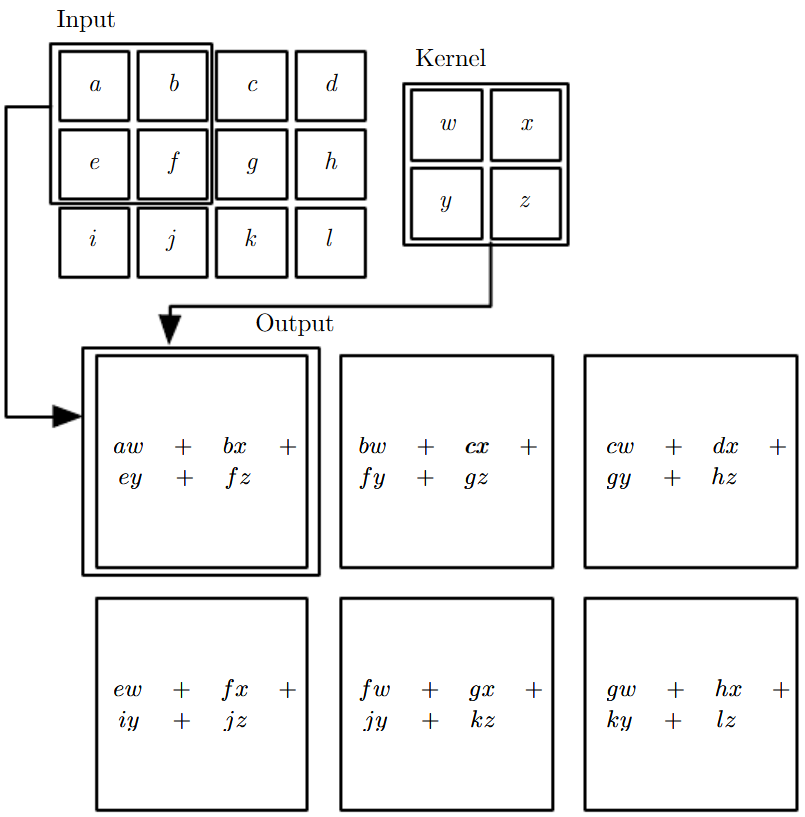
\includegraphics[width=\textwidth]{images/31CNN.png}
		\caption{Príklad 2D konvolúcie s nastaveným jadrom \cite{Goodfellow-et-al-2016}, ktorý sa celý nachádza v obrázku. Niekedy nazývaná ako ``valid'' konvolúcia. Štvorce so šípkami zobrazujú, ako bol vypočítaný horný ľavý element výstupného tenzoru po aplikovaní jadra na príslušný horný ľavý región vstupného tenzora. }
		\label{img:31CNN}
	\end{center}
\end{figure}

V neurónových sieťach je každý element matice váh použitý práve raz pre výpočet výstupu danej vrstvy. Konvolučné neurónové siete majú {\bf zdielané parametre}, čo odkazuje na použitie toho istého parametra vo viac ako jendej funkcii modelu. Namiesto toho, aby sa vypočítala množina parametrov pre každú pozíciu kernelu (každý pixel kernelu je použitý na každom pixeli vstupu), je počítaná jedna množina parametrov pre všetky pozície kernelu.

Forma zdielanaia parametrov pridáva vrstve vlastnosť nazývanú {\bf ekvivariancia}. Funkcie sú ekvivariantné práve vtedy, keď zmenou vstupu sa rovnakým spôsobom zmení aj výstup. Ak máme funkciu $f(x)$ ktorá je ekvivariantá k funkcii $g(x)$, potom musí platiť $f(g(x)) = g(f(x))$. Pre konvolúciu platí: nech $g$ je akákoľvek funkcia, ktorá upraví daný vstup posunom, potom konvolučná funkcia je ekvivariantná ku $g$. Napríklad, nech máme funkciu $I$, ktorá vráti jas obrázka v koordináoch celých čísel. Nech máme funkciu $g$, ktorá mapuje jednu obrázkovú funkciu na inú, teda $I' = g(I)$ je funkcia s $I'(x,y) = I(x - 1, y)$. Takto je posunutý každý pixel obrázka o jednu pozíciu do prava. Ak aplikujeme túto zmenu na $I$ a potom aplikujeme konvolúciu, výsledok bude rovnaký ako pri aplikácii v opačnom poradí, teda konvolúcia na $I'$ a potom zmenu $g$ na výstup konvolúcie. Konvolúcia tvorí teda 2-D mapu výskytu istých vlastností (napr. hrany objektov na obrázku) vstupu. Ak posunieme objekt na vstupe o nejakú hodnotu, výstup bude tiež posunutý o tú istú hodnotu. Pri spracovaní obrázka je napríklad vhodné detegovať hrany na prvej vrstve konvolučnej siete. Rovnaké hrany sa totiž budú vyskytovať v celom obrázku, teda je vhodné zdielať tento parameter po celom obrázku. Môže nastať prípad, keď nie je vhodné zdielať takýto parameter. Príkladom je spracovanie vystrihnutého obrázka a vycentrovaného na tvár, pravdepodobne budeme chcieť rôzne príznaky na rôznych miestach.

Konvolúcia nieje prirozdene ekvivariantná voči niektorím zmenám ako napríklad škálovanie alebo otočenie obrázka. Preto je potrebné aplikovať iné techniky, ako napríklad tzv. augmentácia, na zabezpečenie invariancie voči týmto zmenám. Pri augmentácii ide o úpravu vstupných obrázkov spomínanými zmenami. Takto upravené obrázky sú pridané do vstupného datasetu.

  \subsection{Poolingová vrstva}
Typický modul konvolučnej siete pozostáva z troch stupňov. Prvým je vrstva vykonávajúca paralelne niekoľko konvolúcií a výstupom je množina lineárnych aktivácií. Následne v druhom stupni je na každú lineárnu aktiváciu aplikovaná nelinárna aktivácia ako napríklad usmerňujúca lineárna aktivačná funkcia. Poolingová funkcia na úpravu výstupu vrsty na ďalšie spracovanie je tretí stupeň. 

Poolingová funkcia nahrádza výstup vrstvy na istých miestach štatistickým zhrnutím susedných výstupov (pixelov v prípade spracovania obrazu). Používanými funkciami sú {\bf max pooling}, ktorá aplikuje funkciu nájdenia maximálnej hodnoty medzi susedmi v obdĺžniku daných rozmerov, {\bf average pooling}, ktorá na výstupnú pozíciu uloží priemernú hodnotu susedov v obdĺžniku, {\bf L2 norma} susedov v obdĺžniku alebo {\bf váhovaný priemer} na základe vzdialenosti od centrálneho pixelu.

Na poolingovej vrste sa zvolí jedna z vyššie popísaných funkcií, veľkosť obdĺžnika pre oblasť susedov a krok s ktorým sa obdĺžnik posúva. Daná funkcia je aplikovaná pre každý pixel vstupného obrázka a každý kanál priložením centra obdĺžnika na každý pixel a výpočtom funkcie. Výsledok je uložený príslušnému kanálu na pozíciu centra obĺžnika. Táto vrstva zachováva hĺbku vstupu a zmenšuje šírku a výšku obrázka v závislosti na kroku posunu obdĺžnika.

Vďaka tejto vrstve je reprezentácia invariantná k malým zmenám vstupu. Teda ak sa vstup zmení o malú hodnotu, výstup z poolingovej vrstvy zostáva nezmenený. Invariancia voči lokálym zmenám je použiteľná v prípade, že nás zaujíma výskyt nejakého prízaku a nie jeho umiestnenie v obrázku. Napríklad keď potrebujeme zistiť, či sa na obrázku nachádza tvár, stačí vedieť, že sa oko vyskytuje na ľavej a na pravej strane tváre. \cite{Goodfellow-et-al-2016}

\subsection{Reziduálne učenie}\label{sec:residual}
Kaiming He a kol. \cite{DBLP:journals/corr/HeZRS15} uvažovali hypotézu, že je jednoduchšie optimalizovať tzv. reziduálnu funkciu než pôvodnú funkciu. Ako extrémny prípad, keď je mapovanie identity optimálne, tak je jednoduchšie potlačiť reziduálnu funkciu k nule ako použiť niekoľko nelineárnych funkcií aproximujúcich mapovanie identity.

Uvažujme $H(x)$ ako výstup z niekoľkých po sebe idúcich vrstiev, kde $x$ označuje vstup do prvej vrstvy. Ak existuje hypotéza, ktorá viacerými nelineárnymi vrstvami aproximuje zložitú funkciu, tak potom existuje ekvivalentná hypotéza, ktorá aproximuje reziduálnu funkciu $H(x) - x$. Pričom má vstup aj výstup rovnaké dimenzie. Teda namiesto aproximácie $H(x)$ bude aproximovaná reziduálna funkcia $F(x) := H(x) - x$. Pôvodnú funkciu dostávame výpočtom $F(x) + x$.

\begin{figure}[H]
	\begin{center}
		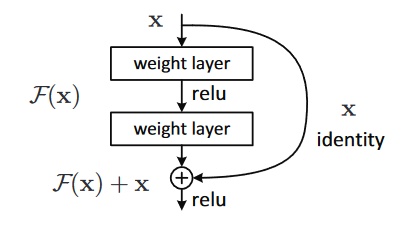
\includegraphics[scale=0.7]{images/residual.png}
		\caption{Reziduálny blok \cite{DBLP:journals/corr/HeZRS15}}
		\label{img:residual}
	\end{center}
\end{figure}

Formulácia $F(x) + x$ môže byť realizovaná doprednov neurónovou sieťou s pridaním "skratky" (Obr. \ref{img:residual}). Spojenia skratkami môžu vynechať jednu alebo viac vrstiev. Vo vetve skratky je použité mapovanie identity, no môže obsahovať ďalšie vrstvy. Výstupy vrstiev sú následne sčítané. He a kol. výskumom ukázali, že siete s reziduálnymi blokmi dosiahli vyššiu presnosť rýchlejšie ako základný model a zvýšením hĺbky siete bola presnosť ešte vyššia.

%\subsection{Hlboké učenie}

\subsection{Architektúra Hourglass}\label{architecture_hourglass}

Návrh hourglass \cite{DBLP:journals/corr/NewellYD16} je motivovaný potrebou zachytenia informácií v každej veľkosti vstupných obrázkov. Niektoré rozmery vrstiev rozpoznávajú príznaky ako napríklad jednotlivé časti tela človeka. Stretávame sa aj s úlohami, kde je potrebné vedieť širší kontext. Napríklad orientácia človeka, usporiadanie končatín a vzťahy medzi susedními kĺbmi. Takéto súvislosti sú najlepšie rozpoznateľné na rôznych škálach obrázka. Hourglass je jednoduchá sieť s minimalistickým návrhom, ktorý má kapacitu zachytiť všetky príznaky a navzájom ich pospájať. Výstupom z takejto siete je pixelová predikcia pravdepodobností.

Pri tejto architektúre je potrebné efektívne spracovať a spojiť príznaky zo všetkých škál. Niektoré prístupy to riešia tak, že nezávisle spracujú obrázok v rôznych škálach a neskôr výstupné príznkay skombinujú. Vďaka reziduálnym vrstvám v hourglass je možné zachovať priestorovú informácia aj pri spracovaní obrázka vo všetkých škálach postupne za sebou.

Postupnosť vrstiev v hourglass je nasledovná: Konvolučné a max pooling vrstvy sú použité na spracovanie príznakov až k najnižšiemu rozlíšeniu obrázka. Na každom max pooling kroku sa sieť rozvetví a aplikuje viac konvolučných vrstiev na obrázok s rozlíšením pred poolingovou vrstvou. Po dosiahnutí najnižšieho rozlíšenia nasleduje upsampling a kombinovanie príznakov na všetkých škálach. Spájanie výstupov z dvoch susedných vrstiev s rôznym rozlíšením je popísané nasledovným postupom podľa Tompon a kol. \cite{DBLP:journals/corr/TompsonJLB14}. Metóda upsampling podľa najbližšieho suseda je aplikovaná na obrázok s menším rozlíšením. Výsledok sa sčíta po pixeloch s pôvodne väčšou vrstvou, ktorá bola vytvorená poolingovími vrstvami zo vstupu. Topológia siete je symetrická. Teda pre každú vrstvu, ktorá sa zmenšuje existuje vrstva, ktoré je vytvorená zväčšením.

Po dosiahnutí výstupného rozlíšenia zo siete sú ešte dve konvolučné vrstvy s jadrom 1x1. Vyprodukujú finálnu predikciu siete formou heatmáp, ktoré reprezentujú pravdepodobnosť výskytu klúčových bodov v každom pixeli. Celý modul je ilustrovaný na Obr. \ref{img:hourglass_architecture}

Nevell a kol. \cite{DBLP:journals/corr/NewellYD16} navrhli implementáciu pri ktorej dospeli k zisteniam, aké možnosti nastavenia vrstiev sú vhodnejšie ako iné. Práca ukázala, že redukčný krok s konvolúciou 1x1 a použitie menších filtrov napomohli k zachyteniu väčšieho priestorového kontextu. Napríklad bolo vhodnejšie použiť dva 3x3 filtre ako jeden 5x5.

\begin{figure}[H]
	\begin{center}
		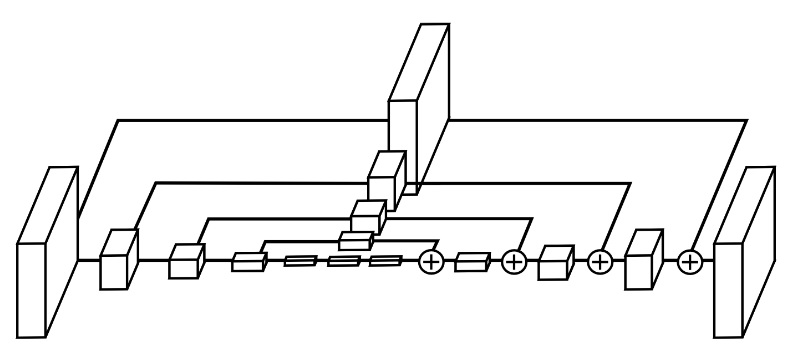
\includegraphics[scale=0.5]{images/hourglass_architecture.jpg}
		\caption{Návrh architektúry hourglass \cite{DBLP:journals/corr/NewellYD16}}
		\label{img:hourglass_architecture}
	\end{center}
\end{figure}

\section{Detekcia pózy ruky konvolučnými sieťami}
V tejto časti popíšeme možnosti pohľadov na riešenie detekcie pózy ruky. Môžeme sa na tento problém pozrieť z pohladu detekcie objektov alebo ako klasifikačný alebo regresný problém. Implementáciou a bližším popisom konkrétnych metód sa budeme venovať v kapitole \ref{chap:previous_solutions}.
\subsection{Detekcia objektov}
Vo všeobecnosti ide pri detekcii objektov o algoritmus, ktorý vytvorí zoznam kategórií objektov nachádzajúcich sa na obrázku a označí všetky nájdené objekty bounding boxom. \cite{Russakovsky2015}

Konvolučná neurónová sieť sa naučií pravdepodobnostnú distribúciu jednotlivých kĺbov. Na výstupe z natrénovaného modelu  sú heat mapy, ktoré obsahujú diskrétne pravdepodobnostné hodnoty kĺbových pozícií. Presnosť odhadovania kĺbov je teda obmedzená rozlíšením heat mapy \cite{Wu18HandPose}. Zoznam kategórií je v tomto prípade reprezentovaný jednotlivými kĺbmi.

\subsection{Regresný prístup}\label{subchapt:regression_approach}
Regresia je typ úloh, ktorý predikuje nejakú numerickú hodnotu pre daný vstup. Na vyriešenie tejto úlohy je použitý učiaci algoritmus s funkciu pre výstup $f: \mathbb{R}^n \mapsto \mathbb{R}$. Ak $y = f(x)$, tak model určí vstupu popísanému vektorom $x$ predikovanú číselnú hodnotu $y$. \cite{Goodfellow-et-al-2016}

Natrénovaná sieť predikuje pozíciu ruky, ktorá je definovaná niekoľkými kĺbmi ruky. Reprezentácia predikcie pre dvojrozmerný vstup je heat mapa pre každý kĺb a pre trojrozmerný vstup je predikcia reprezentovaná relatívnymi 3D koordinátmi ku zápästnému kĺbu. \cite{GANeratedHands_CVPR2018}

\subsection{Klasifikačný prístup}
Klasifikácia odpovedá na otázku, do ktorej kategórie patria vstupné dáta. Riešením takejto úlohy je obvykle použitie učiaceho algoritmu s funkciou $f: \mathbb{R}^n \mapsto \{1, ..., k\}$. Ak $y = f(x)$, tak model určí vstupu popísanému vektorom $x$ kategóriu popísanú číselným kódom $y$. Inou možnosťou je popísať výstup pravdepodobnostnou hodnotou pre každú triedu. \cite{Goodfellow-et-al-2016}

Postupom pri klasifikácii je vytvoriť diskrétny priestor $H$ všetkých možných konfigurácií polohy ruky. Vytvorí sa referenčná databáza $D$, ktorá obsahuje vybrané pózy ruky $\{h_1,h_2,...\} \subseteq H$. Každý vstup do databázy $D$ je dvojica konfigurácie ruky $h$ a vstupného obrázku $I$ prislúchajúcemu tejto konfigurácii: $D = \{(h_1,I_1), (h_2,I_2), ...\}$. Problém je zjednodušený týmto spôsobom na klasifikáciu vstupu, ktorý sa s najväčšou pravdepodobnosťou zhoduje s obrázkom v databáze $D$. Výstupom je potom konfigurácia pózy ruky prislúchajúca tomuto obrázku. \cite{Oikonomidis}

\section{Datasety}\label{datasets}
Na trénovanie neurónovej siete pre nájdenie kľúčových bodov ruky môžeme uvažovať tri možnosti datasetov. Existuje ich niekoľko už vytvorených, ktoré obsahujú obrázky aj s anotáciou klúčových bodov ruky na obrázku. Obrázky sú buď skutočné snímky napr. NYUhands \cite{tompson14tog}, alebo vytvorené modely ľudí s anotovanými rukami napr. RenderedHandposeDataset \cite{zb2017hand}. Treťou možnosťou je vytvorenie vlastného datasetu. V našom prípade kamerou popísanou v časti \ref{camera} uložiť obrázky a priradiť im anotácie. Anotácie v datasetoch sú uvádzané v súradnicovom systéme obrázka tzv. `uvd', kde $u$ a $v$ sú súradnice bodu v pixeloch a $d$ vzdialenosť bodu od ohniska kamery, alebo v kamerovom súradnicovom systéme označovanom ako `xyz'.

\textbf{Dataset NYUhands} \cite{tompson14tog} obsahuje 72 757 trénovacích obrázkov s hĺbkovou mapou. Každý snímok je zachytený troma Kinect kamerami, ktoré sú nasmerované tak, aby snímali osobu z predu, z ľavej a pravej strany. Obrázky zachytávajú jednu osobu. Testovacie dáta obsahujú 8 252 obrázkov dvoch osôb, jedna je rovnaká ako na trénovacích dátach a druhá iná, ktorú sieť ešte nevidela. Všetky obrázky trénovacej aj testovacej množine sú anotované formou uvd a xyz súradníc.

\textbf{Dataset RenderedHandpose} \cite{zb2017hand} obsahuje 41 258 trénovacích a 2 728 testovacích obrákov. V datasete sú RGB obrázky, hĺbková mapa, maska segmentov, 21 kľúčových bodov ruky a nastavenia kamery. Maska segmentov vyjadruje triedy pre pozadie, osobu, tri triedy pre každý prst a jednu pre zápästie. Anotácia kľúčových bodov je reprezentovaná formou uv koordinátov, xyz koordinátov a indikátorom viditeľnosti.

\section{Kamera IntelRealsense d435i}\label{camera}
%Dáta s ktorými budeme pracovať sú produkované kamerou IntelRealsense d435i. 
Kamera poskytuje stereoskopický záznam s hĺbkovou mapou a vďaka malým rozmerom je možná jednoduchá integrácia pre množstvo projektov. 

%\subsection{Hardware}
Kamera zaznamenáva hĺbkovú mapu výpočtami so stereoskopického záznamu. Implementácia tohoto systému pozostáva z ľavej a pravej IR (infračervenej) kamery a IR projektora. IR vysiela neviditeľný IR lúč, čím zvyšuje hĺbkovú presnosť v obraze. Ľavý a pravý snímač zaznamenávajú scénu a dáta odosielajú na vision procesor, kde je vypočítavaná hodnota hĺbky pre každý pixel v obrázku koreláciou bodov ľavého, pravého snímku a ich vzájomnom posune. Hodnoty hĺbkových pixelov vytvoria hĺbkovú mapu pre jeden snímok.

Hĺbkový stereozáznamový modul má dva kamerové senzory {\it OmniVision OV2740} s rovnakým nastevením. Poskytuje maximálne rozlíšenie 1920x1080 v pomere 16:9 alebo 1280x800 v pomere strán 8:5. Minimálna vzdialenosť je 280mm, pre ktorú je možné zaznamenať hĺbku s rozlíšení 1280x720. So znižovaním rozlíšenia minimálna vzdialenosť klesá.

Farebný senzor zaznamenáva RGB obrázok. Pridáva informáciu o textúre hĺbkovému senzoru. Použitím textúry s hĺbkovými dátami je vytvorené farebné mračno bodov použité pri rekonštrukcii 3D modelu zo záznamu.

%\subsection{Uložené dáta}
